\documentclass[a4paper]{scrreprt}
\usepackage{fancyhdr}
\pagestyle{fancy}
\usepackage[english]{babel}
\usepackage[utf8]{inputenc}
\usepackage{graphicx}
\usepackage{url}
\usepackage{textcomp}
\usepackage{amsmath}
\usepackage{lastpage}
\usepackage{pgf}
\usepackage{wrapfig}
\usepackage{fancyvrb}
\usepackage{pdfpages}

\usepackage{etoolbox}
\makeatletter
\patchcmd{\scr@startchapter}{\if@openright\cleardoublepage\else\clearpage\fi}{}{}{}
\makeatother

\newcommand{\code}[1]{\texttt{#1}}

% Create header and footer
\headheight 27pt
\pagestyle{fancyplain}
\lhead{\footnotesize{Applikationer för internet, ID1354}}
\chead{\footnotesize{Assignment 2 report}}
\rhead{}
\lfoot{}
\cfoot{\thepage\ (\pageref{LastPage})}
\rfoot{}

% Create title page
\title{Assignment 2}
\subtitle{Applikationer för internet, ID1354}
\author{Max Körlinge, korlinge@kth.se}
\date{\today}

\begin{document}

\maketitle

\tableofcontents %Generates the TOC
\clearpage

\chapter{Introduction}

This assignment concerns working on the PHP server to implement user authentication, users being able to write comments on recipes, and users being able to delete those comments. Optional tasks were being able to register new users on the site, and storing all recipe data in XML format. I chose to do all tasks (optional and mandatory). I completed the assignment alone.

\chapter{Literature Study}

To complete the tasks I first studied the course lecture notes on the PHP language, PHP for the web server, and XML.

\chapter{Method}

\section{Task 1}

To implement authentication I created a new login page with a form that submits to a PHP script. The script uses the PDO library to make a connection to the mySQL database, which I setup, to check wheither there is a matching username - password entry in the database using a SQL query. I use the \code{\$\_SESSION} variable to store the username and implemented a check in the header included in every page to see if the user is logged in or not. To clarify for the user that there is loading going, on a redirection page was implemented, telling the user what is happening.

\section{Task 2}

The commenting functionality was implemented by including a form at the bottom of the page if the user is logged in (by using the function developed for task 1). The form submits using a PHP script that uses the \code{\$\_POST} and \code{\$\_SESSION} variables to find the comment submitted and the username submitting it, and uses a PDO connection to the mySQL database to store it. While developing this it was also necessery to rework the recipe sites to load comments from the database, instead of hardcoding them as before.

\section{Task 3}

I used the method described in the lecture notes on using hidden input fields in forms to implement being able to delete a comment. The hidden value field is given the \code{recipe\_id} stored in the mySQL database, and then the form submits a script which simply querys the database to delete this entry from the \code{comments} table. While generating the list of comments to the page from the database, the program checks wheither the processed comment was written by the currently logged in user, and then places the delete form next to that comment. No delete button is shown for comments that are not written by the currently logged in user.

\section{Optional Task 1}

To register new users I added a new page for registrations which is very similar to the login page, to keep the design coherent. It uses a similar method to the login page: submitting a form to a PHP script, and the PHP script extracting the new username and password, checking the database for wheither this username already exists (if so returning to the registration page), and if it does not, adding the username and password to the database. The user is then able to log in with the new account.

\section{Optional Task 2}

To store the recipes in XML I used the provided mycookbook template to convert my recipes stored in HTML to properly matching XML tags for this template. I chose to put all recipes in the same XML file, to preserve an order which also could be used to find a matching recipe ID for the database. For example, the first recipe in the XML file has \code{recipe\_id 1} in the database. I used SimpleXML to parse the XML, and rewrote the recipe sites to call a PHP function \code{RecipeSite(\$name)} where you can input the name of a recipe in the database, and it will be output the respective XML contents correctly to the site.


\chapter{Result}
\label{sec:result}

The git repository can be found at https://github.com/fongie/TastyRecipes/tree/assignment2

\section{Task 1}

A login screen is provided (Fig. \ref{fig:login}) and a PHP script checks the mySQL database for a matching username and password combination, as seen in Fig \ref{fig:logincode}. The query will always yield 1 or 0 since usernames are unique in the database, so if it gives a result higher than zero then the user is authenticated. To give user feedback on system status, it is clearly stated that the system is logging you in, until the query is finished. Also, when you are logged in, it clearly says so at the top right of the screen. This is persistent as long as the session is active, since the logged-in script is present in the header of each page.

\begin{figure}[h!]
  \begin{center}
    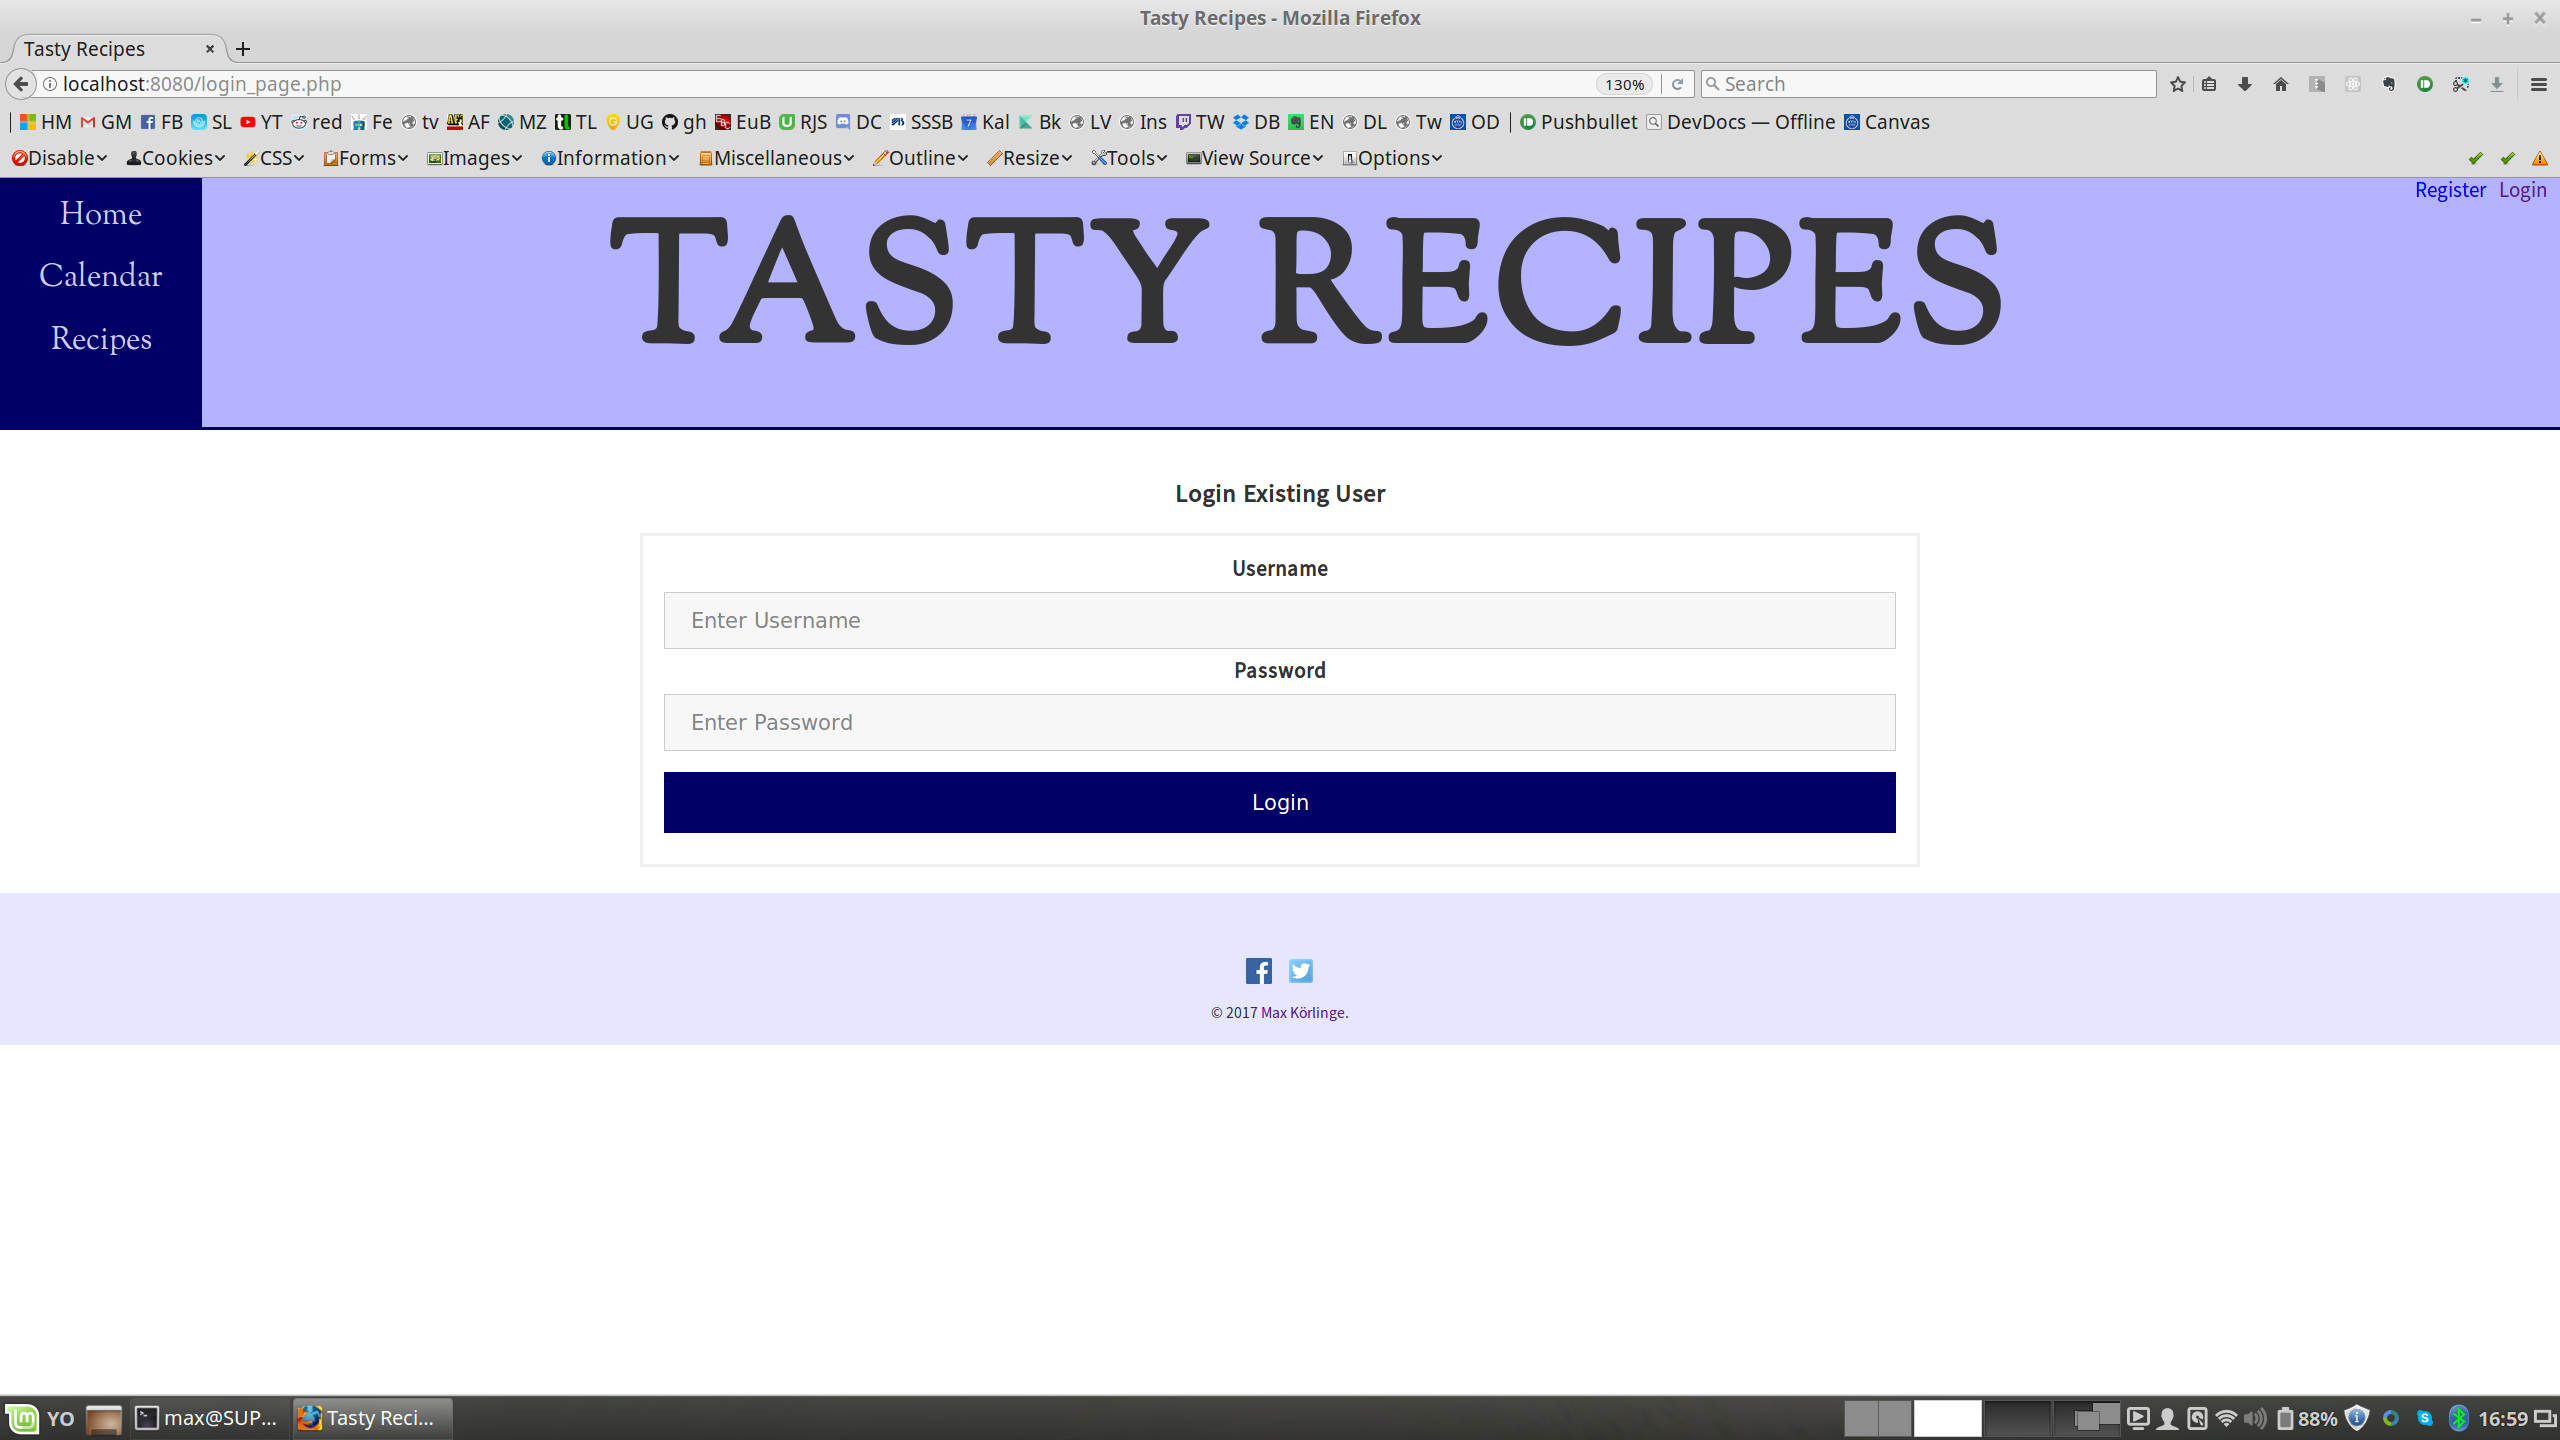
\includegraphics[scale=0.18]{img/login.png}
    \caption{The login page.}
    \label{fig:login}
  \end{center}
\end{figure}

\begin{figure}[h!]
  \begin{center}
    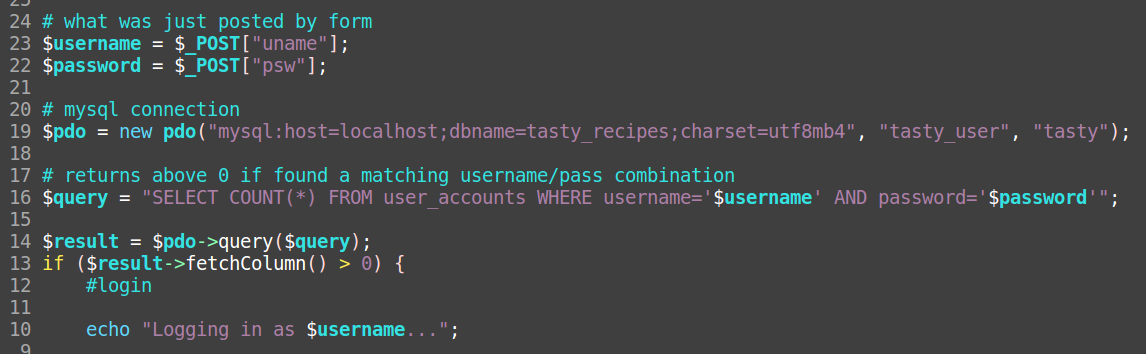
\includegraphics[scale=0.41]{img/logincode.png}
    \caption{Part of the PHP script executing on submitting login form}
    \label{fig:logincode}
  \end{center}
\end{figure}

\section{Task 2}

Comments are fetched from the database and rendered into each recipe page. If the user is logged in, there is also a form at the bottom of the page where the user can enter a comment. The comment is stored in the database together with the user ID who posted it, and the page reloads to show the new comment. The page is shown in Figure \ref{fig:comments}.

The design of the form is in line with the rest of the website, and when a comment is being posted the user is shown a message, so that they know what is going on, to be in line with the heuristics for user design.

\begin{figure}[h!]
  \begin{center}
    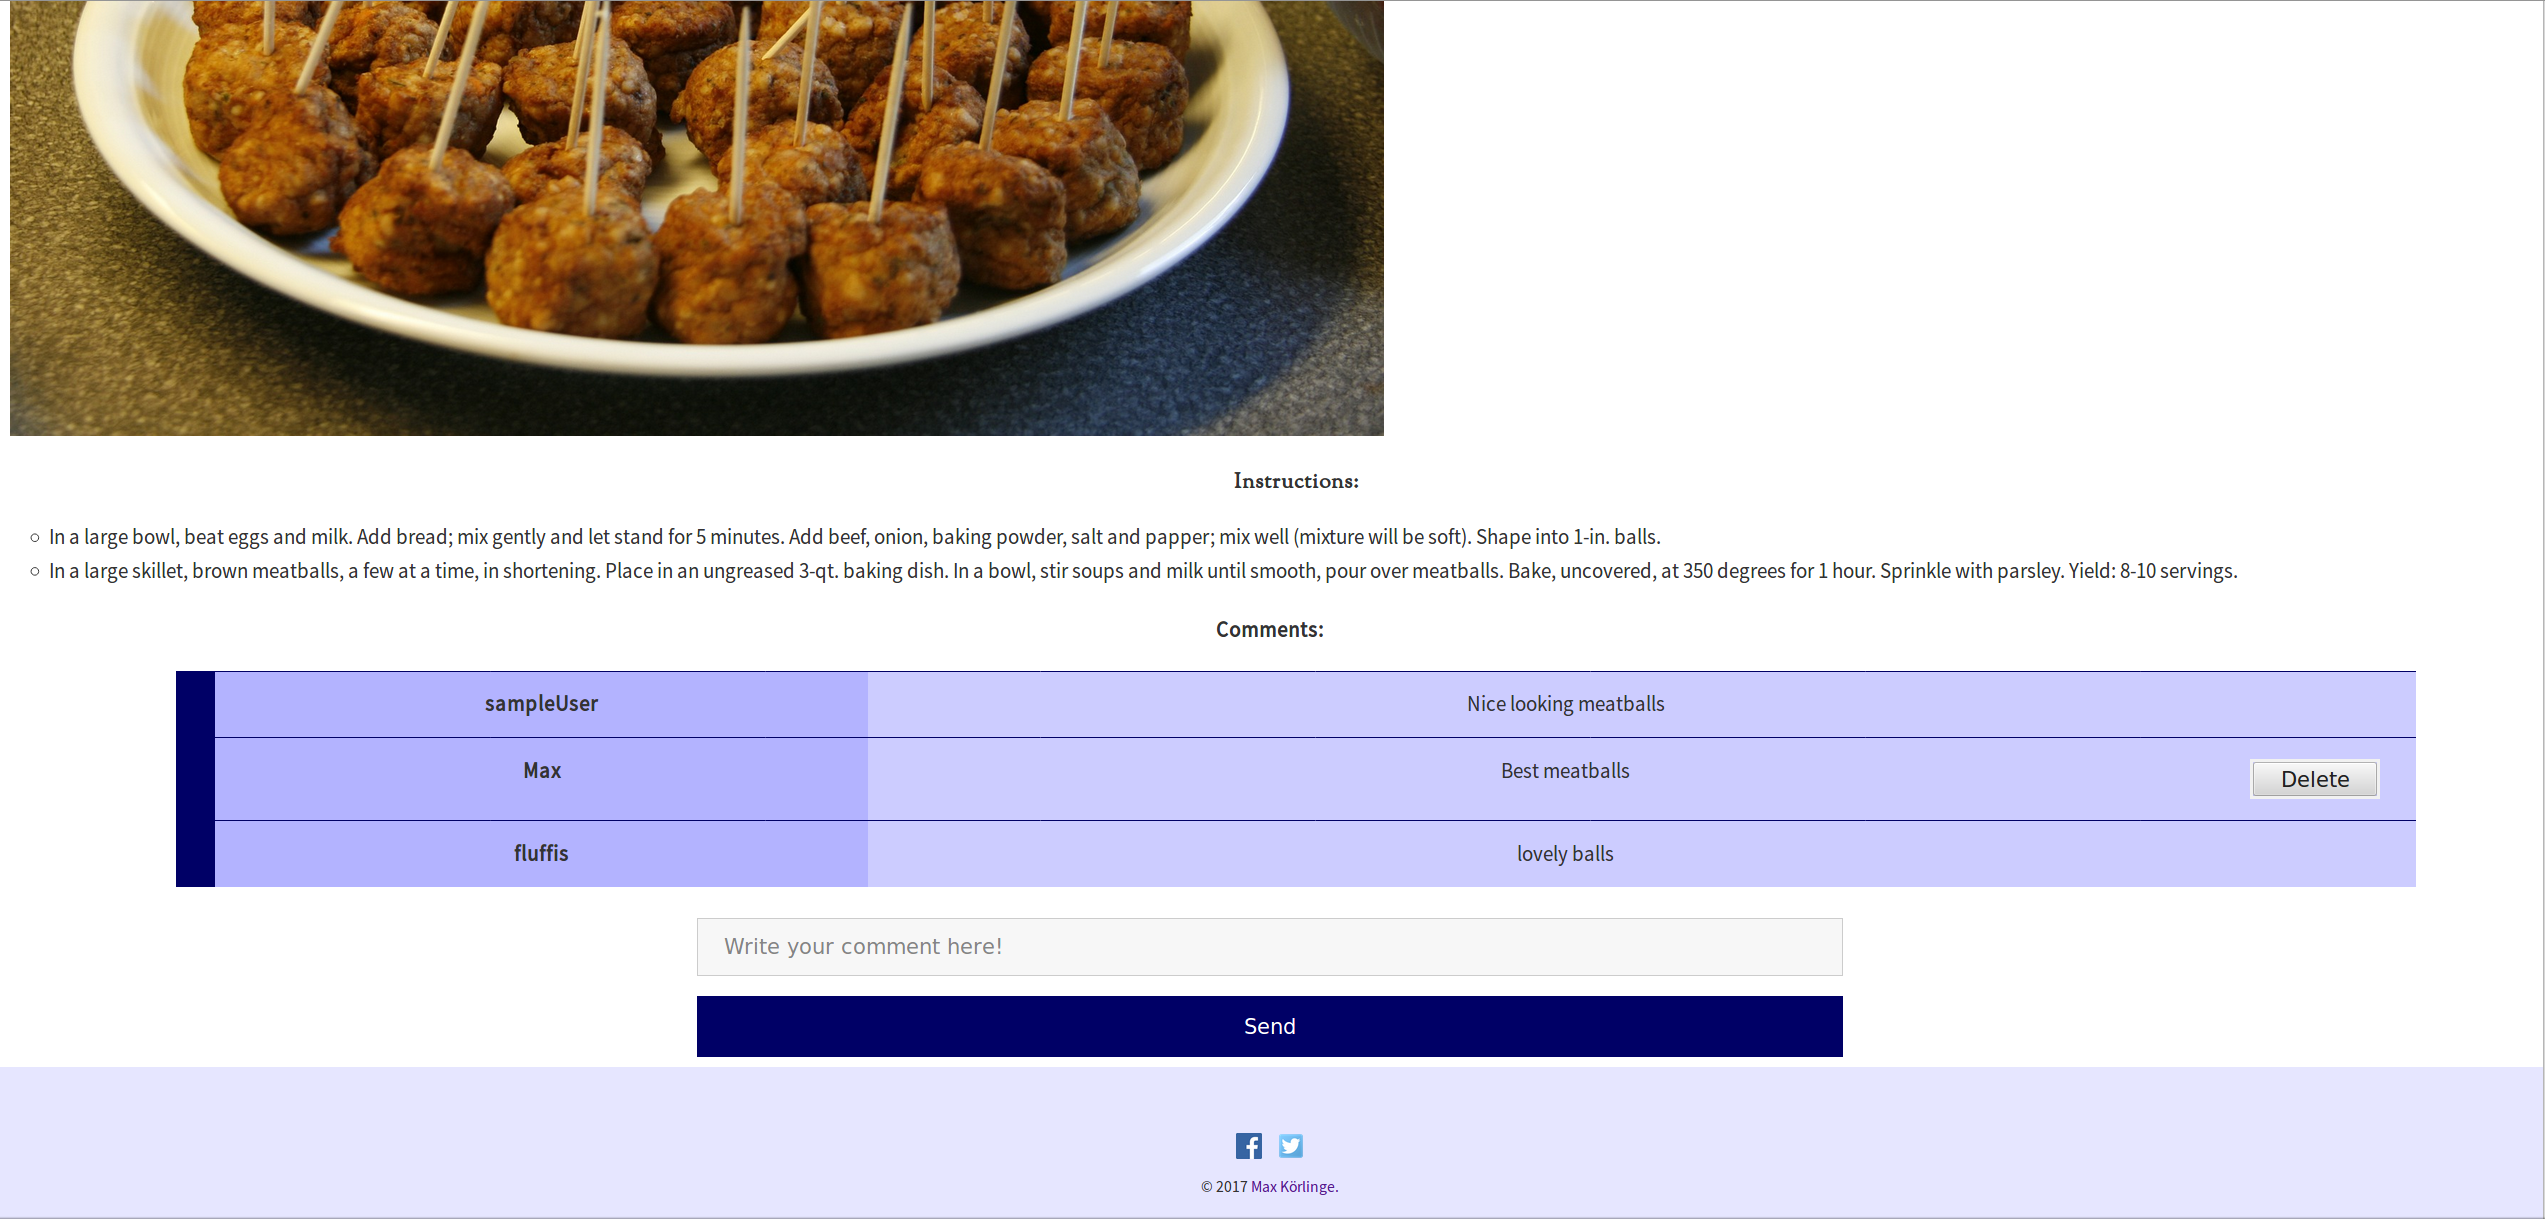
\includegraphics[scale=0.24]{img/comments.png}
    \caption{Comments on the website, showing the form to enter new comment and the option to delete your own comments.}
    \label{fig:comments}
  \end{center}
\end{figure}

\section{Task 3}

As shown in Figure \ref{fig:comments} there is an option to delete one's own comments. As the \code{RecipeSite} function renders all comments from the database, it adds the delete button to comments that have been posted by the same user that is currently logged in (Figure \ref{fig:delete}).

\begin{figure}[h!]
  \begin{center}
    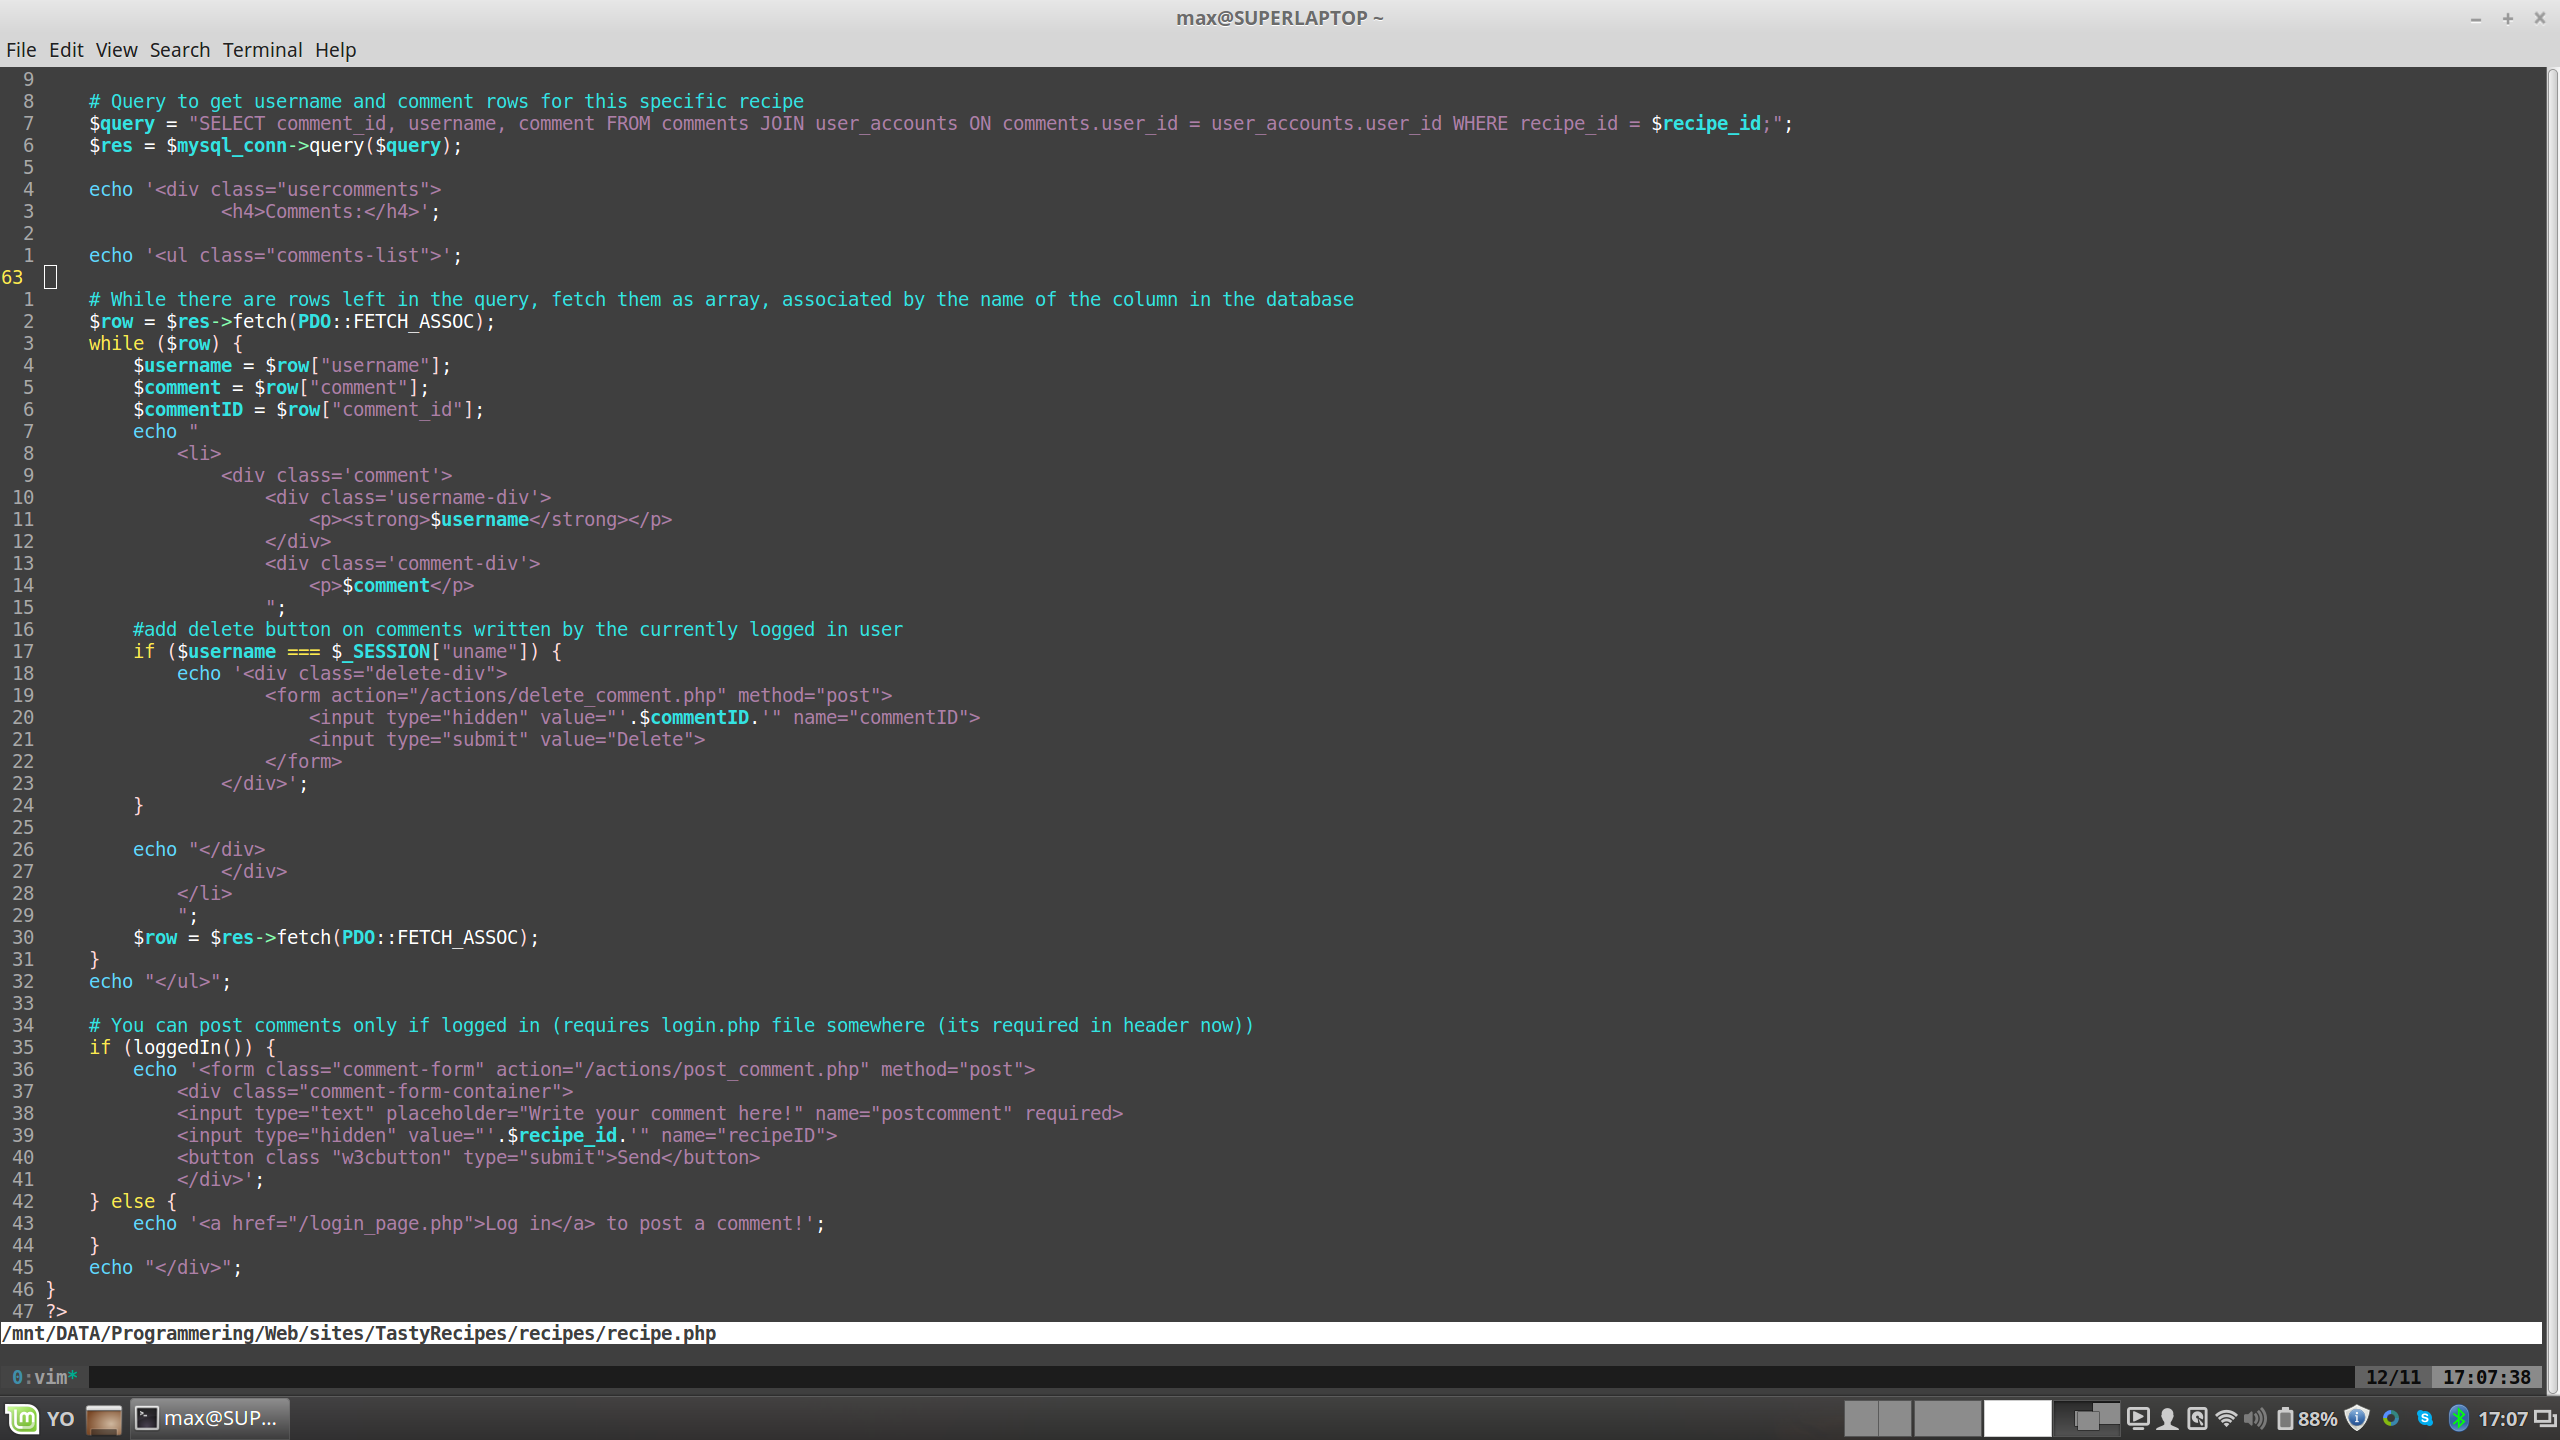
\includegraphics[scale=0.41]{img/delete.png}
    \caption{Code that adds the delete button.}
    \label{fig:delete}
  \end{center}
\end{figure}

\section{Optional Task 1}

New users are registered on a registration page very similar to the login page shown in Figure \ref{fig:login}, only substituting the headline and the input text telling the users to write their own new username and password. If the username does not already exist, it is added to the database by a PHP script using a SQL query shown in Figure \ref{fig:register}. While the request is being processed, the user is shown a message, to clearly state the status of the system.

\begin{figure}[h!]
  \begin{center}
    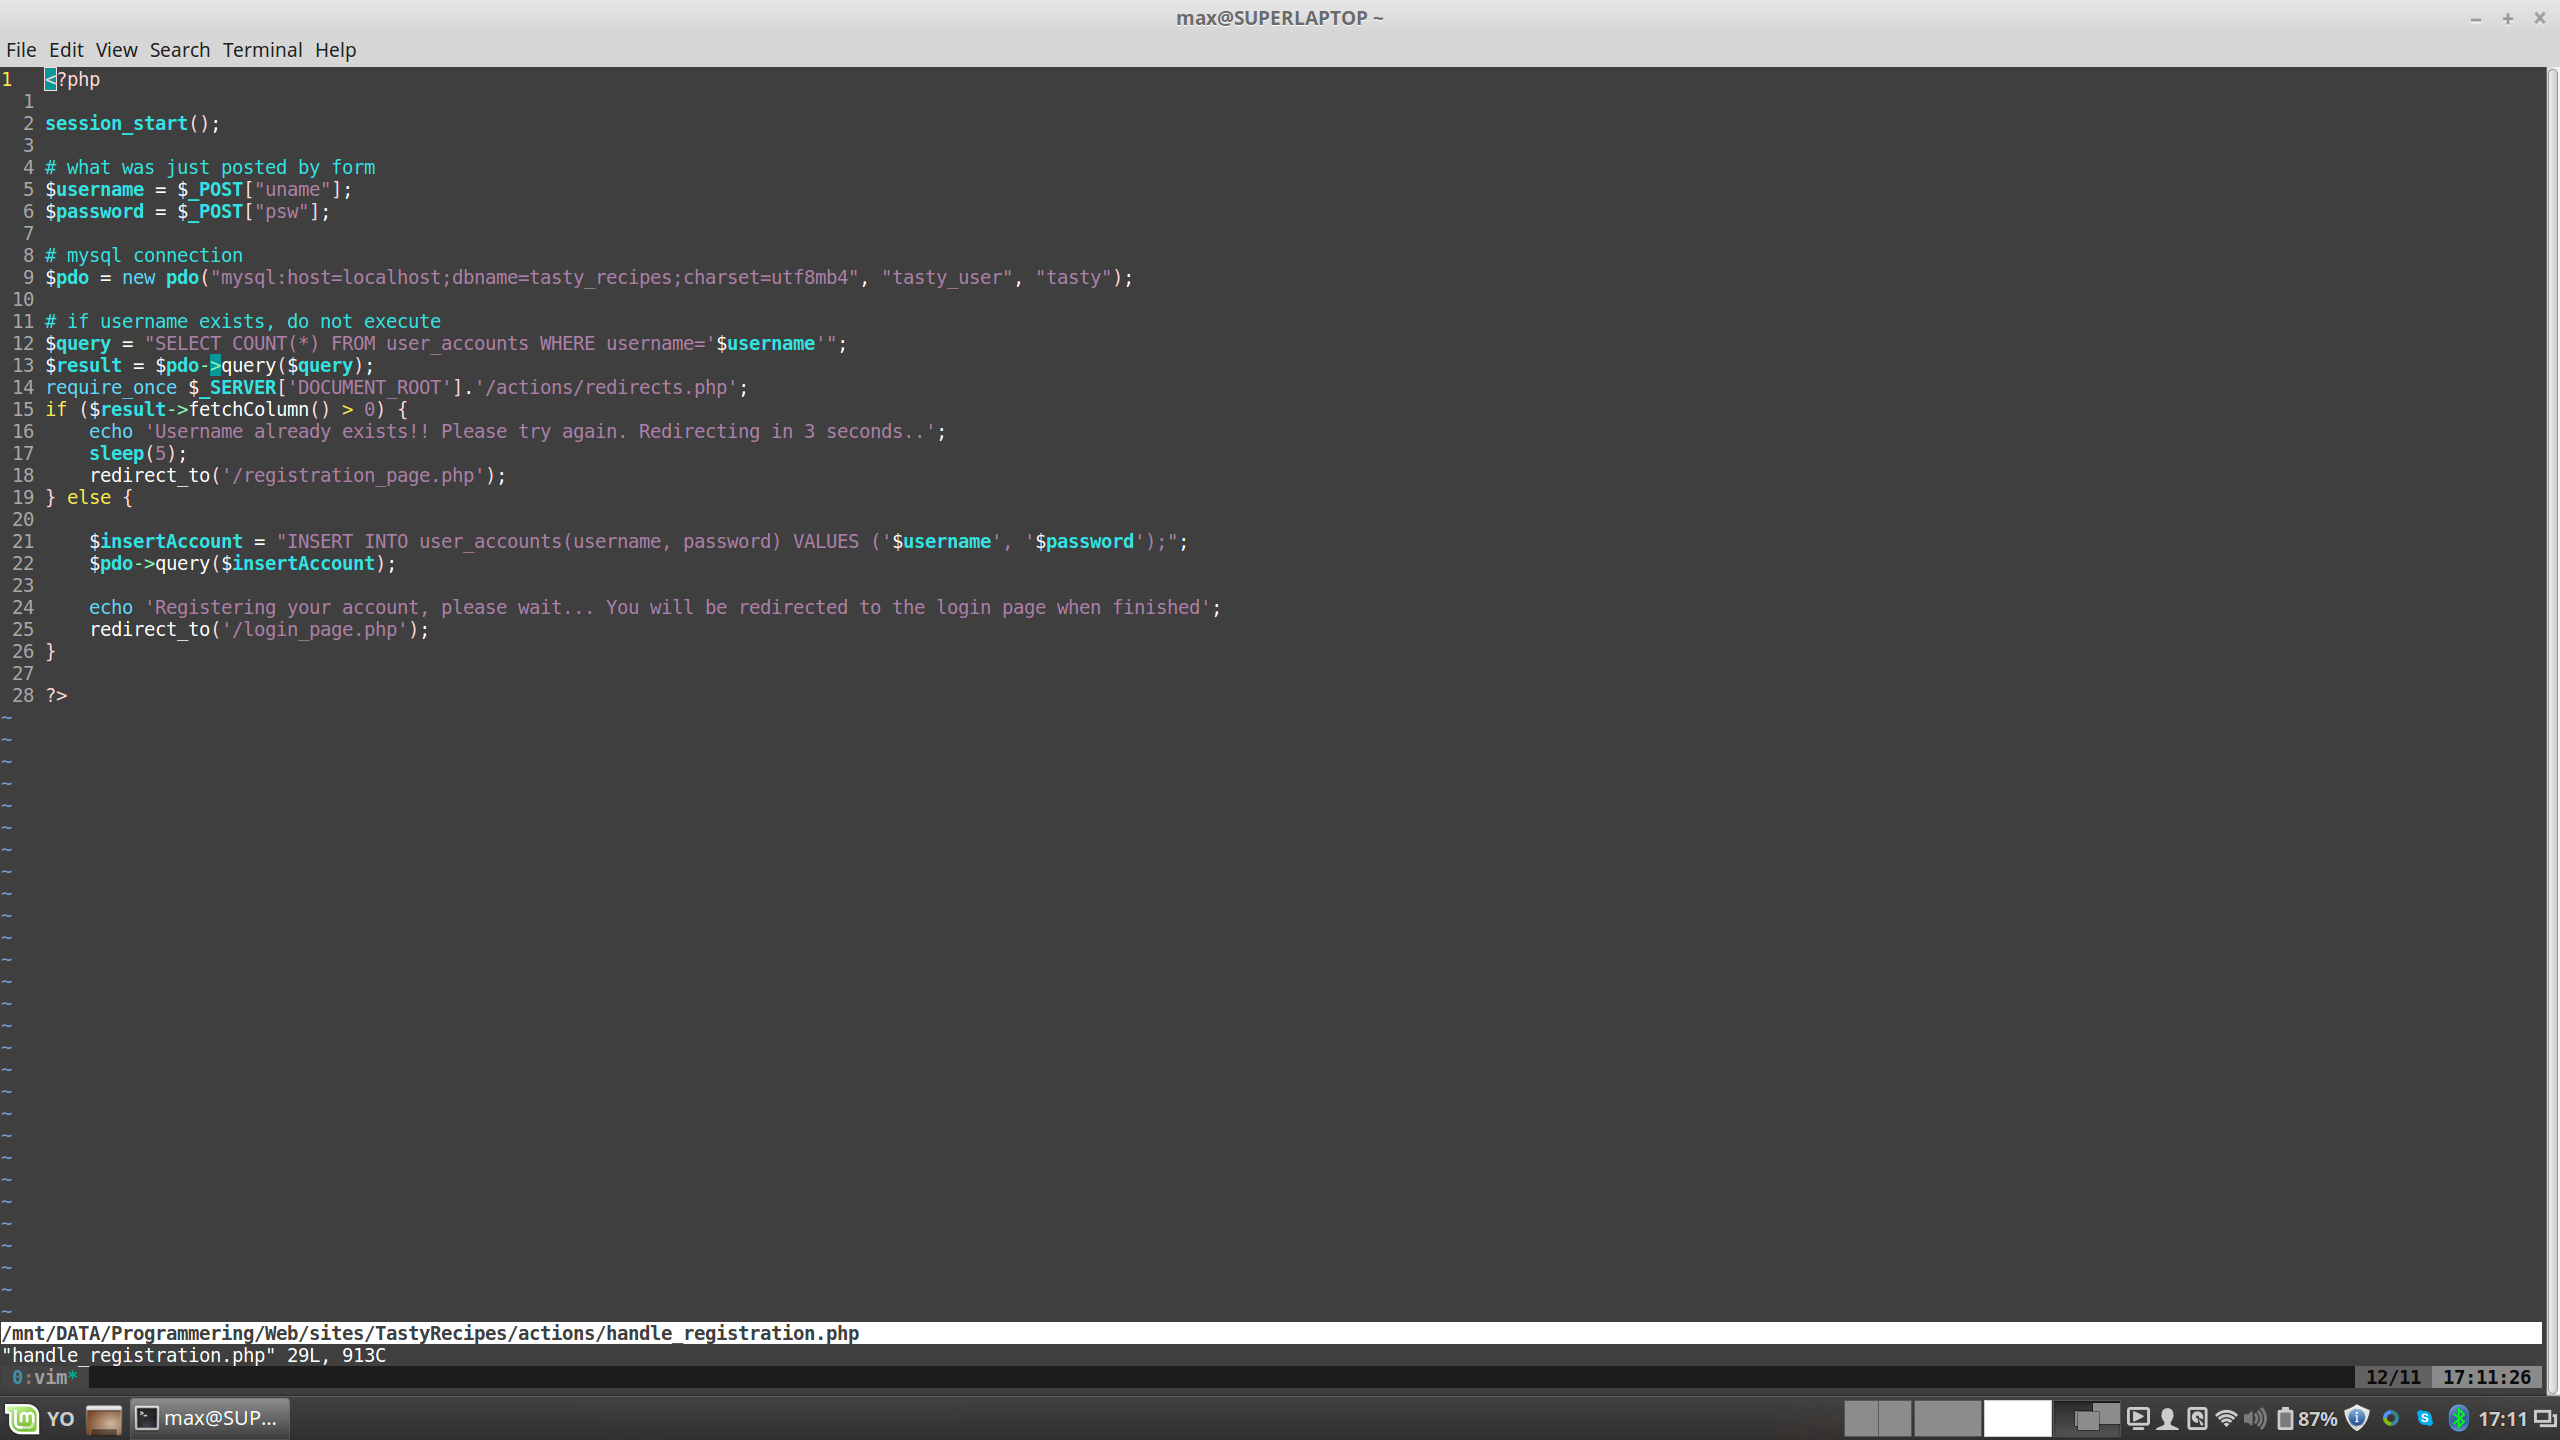
\includegraphics[scale=0.41]{img/register.png}
    \caption{The code that adds the new user to the database.}
    \label{fig:register}
  \end{center}
\end{figure}

\section{Optional Task 2}

Recipes are stored in a single XML file, one after another. It uses the mycookbook template provided in the assignment. The XML is loaded using SimpleXML parser, where you then easily can pick out the values to the keys you want, and render them into the page. This is done in a function called \code{RecipeSite(\$name)} which is called in each recipe site. You can see the part where the XML is parsed to PHP variables in Figure \ref{fig:recipesite}.

\begin{figure}[h!]
  \begin{center}
    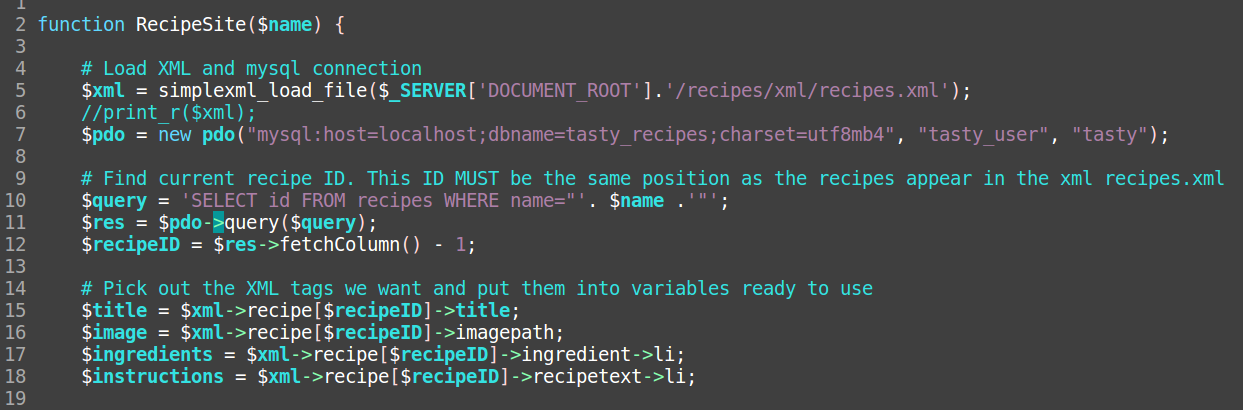
\includegraphics[scale=0.41]{img/recipesite.png}
    \caption{The RecipeSite function which uses XML parsing to find recipe data.}
    \label{fig:recipesite}
  \end{center}
\end{figure}

\chapter{Discussion}

I completed all tasks for this assignment, as shown in the Result chapter above. A requirement throughout the tasks was to keep the five basic heuristics for user interface design fulfilled. In seminar one I found that some of them were hard to apply to those tasks. One of those was the one stating that the user should be shown the status of the system, but this time it has been important to have that in mind since there is more going on server-side. I have solved this design problem by showing the user that they are logged in in the header of the page, and by echoing a message to the user telling them that a request is being processed every time a connection to the database is being made and some loading time could occur, such as when the user logs in, registers, and posts or deletes a comment.

When authenticating the user I decided to use the \code{\$\_SESSION} variable to make the login persist across pages and over the whole browser session. I am aware that you could also accomplish this by using browser cookies, and then you could also have the login persist even after closing down and reopening the browser. I think both ways have merits and accomplish the given task, and my decision to use this method was circumstantial. It would not be difficult to change to using cookies if required at some point.

When dealing with comments on the recipe pages I moved big parts of the recipe pages to PHP functions that dynamically render the data respective to each recipe. I still kept the two pages for the recipes as files in the project, and an improvement to the project would be to render each page according to how many recipes there are in the database, eliminating the need for one PHP file for each recipe. I decided not to do this because of time constraints and because it was not mentioned in the requirements. I did however fulfill the requirements about posting and deleting comments for logged-in users.

I decided early on to use a mySQL database because I wanted to learn how to do it, and also because I know that it is a task in a future assignment. I am also currently studying a course on databases. Because of implementing a database, I think some tasks were easily implemented once that structure was in place and I knew how to interact with it using PHP. For example, deleting comments was as easy as a simple \code{if} clause in the code, together with a one-line SQL query. Also, registering new users was just a short query to insert the data after checking for uniqueness.

Working with XML was not so difficult since it is so similar to HTML, and the SimpleXML parser made it possible to retrieve values through keys corresponding to the XML tags. I used the mycookbook template, but in the end I could remove a majority of the tags and stick with a few ones that seemed appropriate, such as imageURL, recipeText and ingredients. Since no recipe data was then present in the HTML or PHP code, that task was fulfilled as specified.

\chapter{Comments About the Course}

I spent about 30 hours on this assignment, finding it to be quite a large task despite having fiddled around a little in the web world before. It was interesting to finally find out how server side PHP code works. 

I found that working with the code from the first assignment as a starting point lead to very unstructured code at the end of the second, with mixed HTML and PHP code everywhere, despite trying to follow the lecture notes on architecture. I look forward to clean this mess up in the next assignment - since I believe this assignment did not have requirements on code structure.

\end{document}
